\section{Evaluation}
 At this time, we are not aware of any available "gold standard" dataset for hashtag meanings.  In order to compensate, we were forced to create our own test dataset, which consisted of a spreadsheet with 27 hashtags, and known relevant links to each of those hashtags. We understand that this is a small dataset, and not statistically significant, thus is a weak point of our system. Figure \ref{fig:recallat8} shows the results we got for the recall at 8 of the known relevant links that we annotated. We compare our model against a baseline methodology which looks at the top 8 retrieved results when searching the hashtag itself directly on Bing.com. 
\\There are a few takeaways from the results that we say. One important hashtag that our system performs worse in is \#Yosemite, which we annotated links to documents about Apple's newest operating system "Yosemite", but since we tested our evaluated weeks after Yosemite was released, many people were not talking about Apple's OS anymore, and were instead talking about Yosemite National park. Thus, our system returned documents related to the National Park, not the OS. In this way, it is important to note that our system is highly time-dependent for certain hashtags. One of the important properties of hashtags is that their meaning can vary depending on when they are used. In the same regard, our system can perform much better than our baseline method because of the temporal aspect in our system. For example, the hashtag \#LetsGoVCU refers to the Virginia Commonwealth basketball team, who recently made headlines for their game results, and thus there was much talk about them on Twitter using this hashtag. Since LetsGoVCU, is not a common search query, it did not perform well in our baseline. Table \ref{table:recall} shows the average recall at 8 results we achieved.
 
 \begin{figure}[h!]
     \fbox{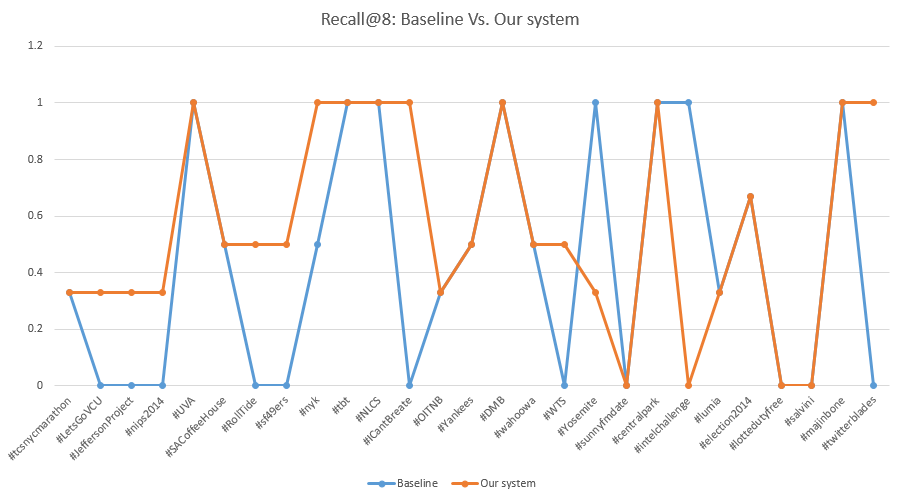
\includegraphics[width=.46\textwidth]{recallat8}}
   \caption{Evaluation results} \label{fig:recallat8}
\end{figure}



\begin{table}[h]
    \centering
    \caption[Table caption text]{Average recall@8.}
    \label{table:recall}
    \begin{tabular}{ | l | l | l |} \hline
    & Baseline & Our system \\ \hline
    Ave. recall@8 & 0.43 & 0.55 \\ \hline
    Matched Hashtags & 16/27 & 23/27 \\ \hline
    \end{tabular}
\end{table}
We did, in addition, do many heuristic based tests to see if we were getting relevant results based on the links that the system returned. We observed that in addition to noisy results, the system did often return at least one or two of the most relevant documents to a particular hashtag. The text summarization aspect did not perform very well, and we attribute this to the fact that in order to generate an accurate summary, the top few links returned must be very relevant to the hashtag, otherwise it will be a completely inaccurate summary.\\